\documentclass[11pt,english,a4paper,parskip=half-]{scrartcl}

\usepackage{mh_basic}
\usepackage{mh_math}
\usepackage{mh_tikz}
\usepackage{mh_theorems}

\usepackage[classic]{agopt_ex}
\usepackage{algorithm}
\usepackage{algpseudocode}
\usepackage{a4wide}
%\textheight25cm

\Lecture{Multicriteria Optimization}
\LectureShort{Multicriteria WS11/12}
\Semester{Wintersemester 2011/12}
\Lecturer{Jun.Prof. Dr. Stefan Ruzika}
\Operator{Dipl.-Math. Michael Helmling}
\Sheetnumber 9
\Homepage{http://optimierung.mathematik.uni-kl.de/teaching/ws1112/multicriteria-opt.html}
\Deadline{January 5th, 2012}
\IssueDate{December 15th, 2011}
\renewcommand{\exercisetext}{Problem}
\InclassDate{December 20th, 2011}
\usepackage{mathtools}
\usepackage{url}
\DeclareMathOperator*{\lexmin}{lex\,min}
\begin{document}
\maketitle

\inclass
\begin{exercise}[\algname{Sum-Max-SPP}]{}
Let $G=(V,A)$ be a directed graph, $s, t \in V$ and denote by
$\mathcal P^{s,t}$ the set of all $s$-$t$ paths in $G$, where a path
$P \in A^{\abs P}$ is defined by its edges.
Consider the following shortest path problem with one sum and $p-1$ bottleneck objectives:
\begin{align*}
\min \,&\left( \sum_{a \in P} c^{1}(a) , \ \max_{a \in P} c^{2}(a), \ \ldots , \ \max_{a \in P} c^{p}(a) \right) \qquad \qquad \tag{\algname{Sum-Max-Spp}}\\[1.2ex]
\text{s.\,t.}\quad & P \in \mathcal P^{s,t}.
\end{align*}
\begin{enumerate}
	\item Find a good upper bound on the number of nondominated points for \algname{Sum-Max-Spp}.
        \item Find an algorithm to find a complete minimal set of efficient solutions. You do not have to give a rigorous proof of the correctness. \emph{Hint: Try to first find a solution for $p=2$, then generalize.}
        \item How can we solve the problem if there are bottleneck objectives only?
\end{enumerate}
\end{exercise}
\begin{solution}
  For a path $P \in \mathcal P^{s,t}$, we define $c^1(P) = \sum_{a \in P} c^1(a)$
  and $c^j(P) = \max_{a \in P} c^j(P)$ for $j=2,\dotsc,p$. For
  $\hat c \in \R^{p-1}$, we define 
  \[\mathcal P^{s,t}_{\hat c} = \left\{ P \in \mathcal P^{s,t}:\,
  c^j(P) \leq \hat c_{j-1} \text{ for }j=2,\dotsc,p\right\} \tp\]
  \begin{enumerate}
	  \item Let $\mathcal X'$ be a minimal complete set of efficient solutions.
	  For each
	  $P \in \mathcal X'$, it must hold that
	  \[c^1(P) = \min\left\{c^1(P'):\,
	  P' \in \mathcal P^{s,t}\text{ with }c^2(P') \leq c^2(P), \dotsc,
	  c^p(P') \leq c^p(P)\right\}\tk\]
	  i.\,e., $P$ must be a minimizer of $c^1$ within $\mathcal P^{s,t}_{(c^2(P),\dotsc,c^p(P))}$. Otherwise, if there were a $P'$ with $c^1(P') \leq c^1(P)$ satisfying
	  all the bottlenecks defined by $P$, that path would dominate $P$. Thus
	  each configuration of bottleneck values contributes at most one element
	  to $\mathcal X'$.
	  
	  Let \[C^j = \{ v \in \R: \exists\, a \in A\text{ with } c^j(a) = v\}\]
	  be the set of distinct cost values of the $j$-th objective function. Then
	  the set of possible configurations of the bottleneck objectives is
	\[ C^1 \times C^2 \times \dotsm \times C^p \]
	and thus $\prod_{j=2}^p \abs{C^j}$ is an upper bound for $\abs {\mathcal X'}
	= \abs{\mathcal Y_N}$. Note
	that $\abs{C^j} \leq \abs A$, so a weaker bound not involving the $C^j$ would
	be $\abs{\mathcal Y_N} \leq {\abs A}^{p-1}$.
	
  We now give an infinite class of graphs for which the first bound is tight.
  Assume $\abs A = k\cdot (p-1)$ for some $k \in \N$ and define 
  $G = (V,A)$ as a line graph with parallel arcs as follows:
  \begin{itemize}
		\item $V = (v_1 = s, v_2, \dotsc,  v_p = t)$
	  \item For each $i \in \{2,\dotsc,p\}$ there are $k$ parallel arcs $(v_{i-1},v_i)$ which we denote by $ a^{i,j}$ for $j=1,\dotsc,k$.
	  \item For an arc $a^{i,j} \in A$, the cost vector is defined by
	  $c^1(a) = -j$, $c^i(a) = j$, $c^l(a) = 0$ for $l \notin \{1,i\}$.
	  An example for $p=4$ and $k=3$ is given below.
  \end{itemize}
	\begin{center}
		\begin{tikzpicture}
			\node[v] (1) at (0,0) {$s$};
			\node[v] (2) at (3,0) {$v_2$};
			\node[v] (3) at (6,0) {$v_3$};
			\node[v] (4) at (9,0) {$t$};
			\draw[a] (1) to[bend left=50] node[above] {$(-1,1,0,0)$}(2);
			\draw[a] (1) to[bend left=0] node[above] {$(-2,2,0,0)$} (2);
			\draw[a] (1) to[bend right=50] node[below] {$(-3,3,0,0)$} (2);
			
			\draw[a] (2) to[bend left=50] node[above] {$(-1,0,1,0)$}(3);
			\draw[a] (2) to[bend left=0] node[above] {$(-2,0,2,0)$} (3);
			\draw[a] (2) to[bend right=50] node[below] {$(-3,0,3,0)$} (3);

			\draw[a] (3) to[bend left=50] node[above] {$(-1,0,0,1)$}(4);
			\draw[a] (3) to[bend left=0] node[above] {$(-2,0,0,2)$} (4);
			\draw[a] (3) to[bend right=50] node[below] {$(-3,0,0,3)$} (4);
		\end{tikzpicture}
	\end{center}
	We claim that $\mathcal P^{s,t}$ is a minimal efficient set, i.\,e.\ all
	paths are efficient and have different objective values. As for the latter,
	observe that the choice of the $i$-th arc of a path, $a^{i,j}$,
	uniquely determines
	$c^{i+1}(P)$, because $a^{i,j}$ is the only arc $a \in P$ with 
	$c^{i+1}(a) \neq 0$. Because $c^{i+1}(a^{i,j})$ is different for all
	$j=1,\dotsc,k$, all paths have different costs in the bottleneck
	objectives.
	
	To show that all paths are efficient, assume for the contrary that
	a path $P$ is dominated by some other path $\hat P \neq P$.
	Let $i$ be minimal such that $P \ni a^{i,j} \neq a^{i,\hat j} \in \hat P$,
	i.\,e.\ the paths differ in the $i-1$-st arc. Since $\hat P$ dominates $P$,
	we must have $\hat j < j$, otherwise $c^i(P) = j < c^i(\hat P) = \hat j$ and 
	$P$ would not be dominated.
	
	But then $c^1(a^{i,\hat j}) > c^1(a^{i,j})$,
	so there must be at least one index $i' > i$ where $\hat P$ takes an arc
	with larger index: $P \ni a^{i', j'} \neq a^{i', \hat j'} \in \hat P$
	with $\hat j' > j'$. This however implies $c^{i'} (P) < c^(i')(\hat P)$,
	which is a contradiction to $\hat P$ dominating $P$.
	
	\item We claim that \prettyref{alg:summaxspp} computes a minimal efficient
	set for \algname{Sum-Max-Spp}. Observe that the \textbf{for} loop
	in \prettyref{line:forloop} traverses all possible configurations of the bottleneck costs. Thus,
	by the argumentation of part~a), the total set of paths generated in
	\prettyref{line:genpath} contains a minimal complete efficient set. It is 
	left to show that the detection of dominated solutions in the following lines
	is correct; i.\,e.\ that in \prettyref{line:solutionincrease}, we add exactly
	one path for each $y \in \mathcal Y_N$.
	
	\begin{lemma}
	For $\hat c \in C^2 \times \dotsm \times C^p$, let
	\[c^*(\hat c) = \min_{P \in \mathcal P^{s,t}_{\hat c}} c^1(P)\text{ and }
	P^*(\hat c) = \argmin_{P \in \mathcal P^{s,t}_{\hat c}} c^1(P)\tk\]
	if such a path exists. Then the set \[ \mathcal P_{\mathtt{Alg}}\left\{P^*(\hat c):  
	\mathcal P^{s,t}_{\hat c} \neq \emptyset,\; c^*(\hat c') > c^*(\hat c)\text{ for all }
	\hat c' \leq \hat c,\; \hat c' \neq \hat c\right\}\]
	is a minimal complete set of efficient solutions for \algname{Sum-Max-Spp}.
	\end{lemma}
	\begin{proof}
	Let $P \in \mathcal X_E$ be an efficient path with objective value
	$c(P) = c^1(P), \dotsc, c^p(P)$. Let $\hat c = (c^2(P), \dotsc, c^p(P))$, then
	by part~a), $c(P) = c^*(\hat c)$. Assume that $\mathcal P_{\mathtt{Alg}}$ does
	not contain any path $P'$ with $c(P') = c(P)$. Then by definition of
	$\mathcal P_{\mathtt{Alg}}$ there must be some $\hat c' \leq \hat c$
	such that $c^*(\hat c') \leq c^*(\hat c)$. But this means that $P^*(\hat c')$ 
	dominates $P$, contradicting $P \in \mathcal X_E$.
	\end{proof}
	With the additional observation that for any $\hat c' \geq \hat c$ we necessarily have $c^*(\hat c') \leq  c^*(\hat c)$ (since constraints are relaxed)
	it is easy to see that \prettyref{alg:summaxspp} computes $\mathcal P_{\mathtt{Alg}}$ and is thus correct.
	
	Its running time is, if we omit output cost in \prettyref{line:solutionincrease},
	$\O\left( \prod_{j=2}^p \abs{C^p}\left(\abs V \log \abs V + \abs A\right)\right)$: The shortest path computation in 
	\prettyref{line:genpath} can be accomplished in
	$\Theta\left(\abs V \log \abs V + \abs A\right)$ using Dijkstra's algorithm
	with Fibonacci heaps. Disabling arcs that don't meet the bottleneck constraints
  $\hat c$ takes only linear time for each such $\hat c$. 
  \item When there are bottleneck objectives only, we could use a modification
  of \prettyref{alg:summaxspp} to compute a minimal complete efficient set.
  Instead of the minimum $c^1$-values for each bottleneck configuration,
  however, the \texttt{Value} array only needs to store a boolean flag,
  whether there exists a path in $\mathcal P^{s,t}_{\hat c}$ or not. Thus
  in \prettyref{line:genpath} we can use a linear-time connectedness test
  instead of shortest path computation. 
  The following observations could be used to further reduce the running
  time:
  \begin{itemize}
    \item a path with objective
  value $c(P) = c^1(P),\dotsc,c^p(P)$ is efficient if and only if there does not
  exist a path $P'$ with $c(P') \leq c(P),\; c(P') \neq c(P)$;
    \item if $\mathcal P^{s,t}_{\hat c}$ is empty for some $\hat c$, then it is also empty
  for every $\hat c' \leq \hat c$;
    \item  if $\mathcal P^{s,t}_{\hat c}$ is nonempty, that also holds for all $\hat c' \geq \hat c$.
  \end{itemize}
  \end{enumerate}
\begin{algorithm}[H]
	\begin{algorithmic}[1]
	\State\textbf{Input:} Graph $G=(V,A)$ with $p$ objective functions $c^1,\dotsc,c^p$.
	\State\textbf{Output:} A minimal complete set $\mathcal S$ of efficient solutions for \algname{Sum-Max-Spp}.
	\ForAll{$j=2,\dotsc,p$}
		\State Compute and $C^j$ and sort it such that $C^j_1 \leq \dotsi \leq C^j_{\abs{ C_j}}$
	\EndFor
	\State Allocate a $p-1$-dimensional array
		\texttt{Value}$\left[\abs{C^2},\dotsc,\abs{C^p}\right]$
	\State $S \gets \emptyset$
	\ForAll{$I \in \left[1,\abs{C^2}\right] \times \dotsm \times \left[1,\abs{C^j}\right]$, traversed in lexicographic order}\label{line:forloop}
		\State $\hat c \gets (C^2_{I_1}, \dotsc, C^p_{I_{p-1}})$
		 \label{line:genpath}
		\State Find a path $P = \argmin_{P \in \mathcal P^{s,t}_{\hat c}} c^1(P)$
		\If{there is no such path ($\mathcal P^{s,t}_{\hat c}$ is empty)}
			\State \texttt{Value}$[I] \gets \infty$
		\Else
			\State \texttt{Value}$[I] \gets c^1(P)$
			\State \texttt{dominated} $\gets $ \texttt{False}
			\ForAll{$i=1,\dotsc,p-1$ with $I_i > 1$}
				\State $\hat I \gets I$
				\State $\hat I_i = \hat I_i - 1$
				\If{\texttt{Value}$[\hat I] = c^1(P)$}\label{line:dominatetest}
					\State \texttt{dominated} $\gets $ \texttt{True}
					\State\textbf{break}
				\EndIf
				\If{not \texttt{dominated}}
					\State $S \gets S \cup \{P\}$ \label{line:solutionincrease}
				\EndIf
			\EndFor
		\EndIf
	\EndFor
	\State	\Return $S$
	\end{algorithmic}
	\caption{Algorithm solving \algname{Sum-Max-Spp}}\label{alg:summaxspp}
	\end{algorithm}
\end{solution}

\takehome

\begin{exercise}{}\label{ex:bla}
\begin{figure}[ht]
\center
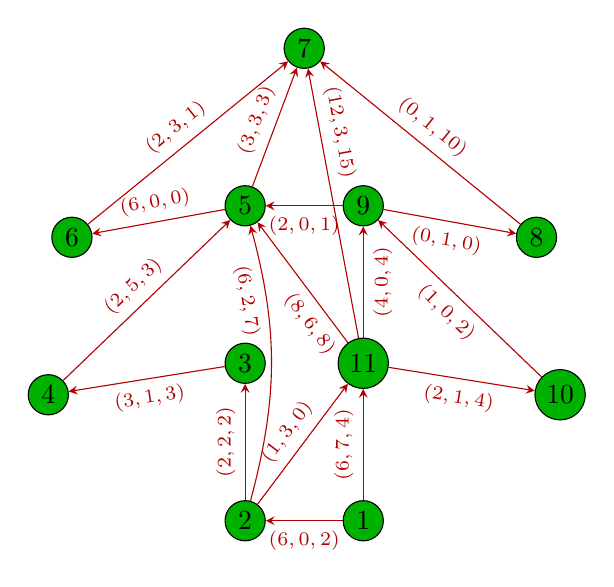
\begin{tikzpicture}[v/.append style={draw,circle,inner sep=.8mm,minimum size=3mm,fill=green!70!black},
					a/.append style={->,>=stealth,font=\scriptsize,sloped,color=red!70!black}]
\node[v] (1) at (1.5,0) {1};
\node[v] (2) at (0,0) {2};
\node[v] (3) at (0,2) {3};
\node[v] (4) at (-2.5,1.6) {4};
\node[v] (5) at (0, 4) {5};
\node[v] (6) at (-2.2, 3.6) {6};
\node[v] (7) at (.75, 6) {7};
\node[v] (8) at (3.7, 3.6) {8};
\node[v] (9) at (1.5,4) {9};
\node[v] (10) at (4, 1.6) {10};
\node[v] (11) at (1.5,2) {11};
\draw[a] (1) -- node[below] {$(6,0,2)$}  (2);
\draw[a] (1) -- node[above] {$(6,7,4)$}  (11);
\draw[a] (2) -- node[above] {$(2,2,2)$}  (3);
\draw[a] (2) to [bend right=15] node[below,near end] {$(6,2,7)$}  (5);
\draw[a] (2) -- node[above] {$(1,3,0)$} (11);
\draw[a] (3) -- node[below] {$(3,1,3)$} (4);
\draw[a] (4) -- node[above] {$(2,5,3)$} (5);
\draw[a] (5) -- node[above] {$(6,0,0)$} (6);
\draw[a] (5) -- node[above] {$(3,3,3)$} (7);
\draw[a] (6) -- node[above] {$(2,3,1)$} (7);
\draw[a] (11) -- node[below,near start] {$(8,6,8)$} (5);
\draw[a] (11) -- node[above,near end] {$(12,3,15)$} (7);
\draw[a] (11) -- node[below,swap] {$(4,0,4)$} (9);
\draw[a] (11) -- node[below] {$(2,1,4)$} (10);
\draw[a] (10) -- node[below] {$(1,0,2)$} (9);
\draw[a] (9) -- node[below] {$(2,0,1)$} (5);
\draw[a] (9) -- node[below] {$(0,1,0)$} (8);
\draw[a] (8) -- node[above] {$(0,1,10)$} (7);
\end{tikzpicture}
\caption{The graph for \prettyref{ex:bla}}\label{fig:christmas}
\end{figure}
\begin{enumerate}
\item Using the multicriteria label-setting algorithm from the lecture, compute
a minimal complete set of efficient paths from $v_1$ to $v_7$ in the graph of
\prettyref{fig:christmas}.
\item Consider a directed graph $G=(V,A)$ with cost function $c:\, A \rightarrow \R^{p}$ not containing negative cycles, i.\,e., for all cycles $Z$ in $G$ we have $c(Z) = \sum_{a \in Z}c(a) \geq 0$.
  \begin{enumerate}
  \item Prove the following statement:    
   Let $P^{s,t}$ be an efficient $s$-$t$ path on $G$. Then any subpath $P^{u,v}$ from $u$ to $v$, where $u$ and $v$ are vertices on $P^{s,t}$, is an efficient path from $u$ to $v$.
  \item Show that the converse is not true in general, i.\,e.\ compositions of efficient paths are not necessarily efficient.
  \end{enumerate}
\end{enumerate}
\end{exercise}

\begin{exercise}[Multicriteria \algname{FloydWarshall}]{}
Recall how the algorithm of Floyd and Warshall computes all-to-all shortest paths in a directed graph under the assumption that it does not contain negative dicycles. The objective of this exercise is to extend that algorithm so as to find a minimal complete efficient set for a multicriteria shortest path problem (which also must not contain any negative cycle in the sense of \prettyref{ex:bla}).

To solve this exercise, assign a list of labels to each node, similar as for the multicriteria label-setting algorithm in the lecture. Then use the generalized Bellman principle of the previous exercise to restrict the set of possible efficient paths in the inner \texttt{FOR} loop of \algname{FloydWarshall}. 
\end{exercise}
\end{document}
